%%% fs-seim-typical - Typical solutions

\label {fs-typical}

There are two common methods that are used to implement order-sensitive operators: in-order processing (IOP) \cite{Arasu:2006:CCQ:1146461.1146463} \cite{Cranor:2003:GSD:872757.872838} \cite{hammad2004optimizing} and out-of-order processing (OOP)\cite{Li:2008:OPN:1453856.1453890}.

\subsection{IOP}

In IOP approach each operation enforces total order on elements. For example union combines multiple streams into one \ref{iop}. Each input stream of union is ordered, as predecessors must meet ordering constraint. If there is arrival time skew between input stream, union must buffer the earlier stream to produce ordered output. Operators such as projection and selection applies function and propagete items down the stream without any additional buffering.

\begin{figure}[htbp]
  \centering
  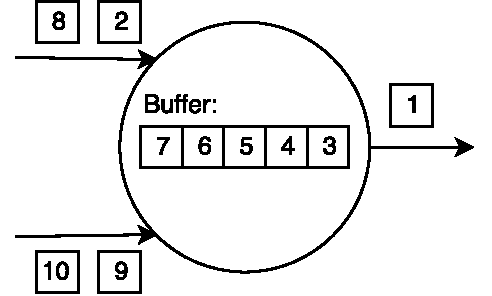
\includegraphics[width=0.30\textwidth]{pics/iop}
  \caption{IOP union operation. Due to delay of the first stream operation must buffer elements}
  \label {iop}
\end{figure}

IOP is know to be memory demanding, to have unpredictible latencies and limitid scalability.\cite{Li:2008:OPN:1453856.1453890}

\subsection{OOP}

OOP is an architecture of streaming systems that doesn't require order maintaince. To unblock blocking operations OOP systems use progress indicators such as punchuations \cite{Tucker:2003:EPS:776752.776780}, low watermarks \cite{Akidau:2013:MFS:2536222.2536229} or hearbeats \cite{Srivastava:2004:FTM:1055558.1055596}. Punctuations are periodically yielded by data sources and carries timestamp that promises that there won't be any elements older that punctuation's value. Punctuations are monotonic and data items between two consecutive punctuations can be arbitrarily reordered. Operations propagates them with respect to their semantics.

\begin{figure}[htbp]
  \centering
  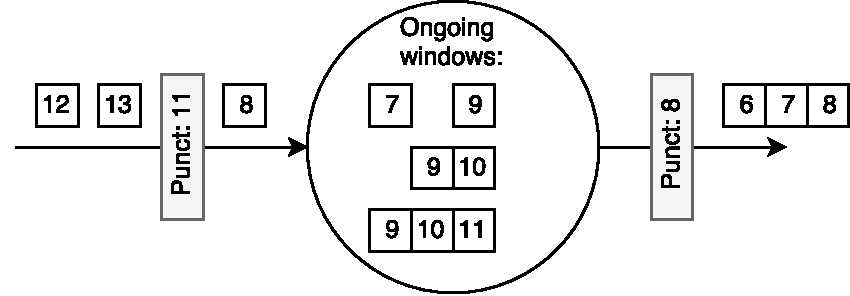
\includegraphics[width=0.48\textwidth]{pics/oop}
  \caption{OOP sliding window, range=3, slide=1. Operation must block last window until next punctuation arrival }
  \label {oop}
\end{figure}

For example, windows collects partial aggregates until punctuation that guarantees that there are no elements can be delivered to the window's input that belog to the ongoing window.  On punctuation's arrival it flushes completed windows and propagates punctuation to the next operation down the stream \ref{oop}

OOP resolves some of the downsides of IOP but it has several flaws. Even if the input stream is totally ordered, operation must wait the punctuation to guarantee it. Another issues is that periodial flushes can result in load bursts. This can result in latency increase.
